
\subsection{The Filesystem}

We model a working filesystem
using a function $\FS$ with a set of nodes (filesystem paths) $\setn$ as its domain,
and a set of possible contents or values $\setv$ as its codomain.
Alternatively, if the filesystem has encountered a problem and is no longer usable, 
we assign it the special value $\fsbroken$:
\begin{mydef}[Filesystem]
\begin{gather*}
\FS =
\begin{cases}
\setn \rightarrow \setv \\
\fsbroken
\end{cases}
\end{gather*}
\end{mydef}
In our model, $\setn$ 
serves as a namespace or ``skeleton'' for the filesystem.
It contains all possible nodes, including the ones 
where the file system contains no file or directory,
where in our model $\FS$ has a special value, $\empt\in\setv$.

The nodes form a disjoint union of rooted directed trees,
which determines the following $\parent$ function,
and \emph{ancestor / descendant} and \emph{incomparable} relations.
Tao et al. in \cite{TSR} describe a similar filesystem model, although
they also model inodes and restrict the filesystem to a just single tree.
\begin{mydef}[$\parent$]
The function $\parent(n)$ returns the parent node of $n$, or
returns $\topnode$ if $n$ is the root of a tree.
\end{mydef}

\begin{mydef}[$n\descendant m$]
On $\setn$ the \emph{ancestor / descendant} relation is the
partial ordering determined by the $\parent$ function.
We write $n\descendant m$ if $n$ is the ancestor of $m$,
that is, $n=\parent^n(m)$ for some integer $n\ge 1$.
% or the path name of $n$ is an initial segment of that of $m$. 
We write $n\descendantEq m$ if $n\descendant m$ or $n=m$.
\end{mydef}

\begin{mydef}[$n\unrel m$]
We write $n\unrel m$, or $n$ and $m$ are \emph{incomparable}
if $n\not\descendantEq m$ and $n\not\ancestorEq m$;
that is, incomparable nodes are on different branches or on different trees.
% none of the path names describing their location is an initial segment of the other.
\end{mydef}

Every working filesystem has a so-called \emph{tree property}, which means that
if the filesystem is not empty at a node, and the node has a parent,
then there must be a directory at the parent node.
To model this, in $\setv$ we select another special value
to represent directories, as we assume that apart from their location
in the filesystem, all directories are equal.
We do this because, as Bill Zissimopoulos pointed 
out (\cite{BZ}),
we often do not want to consider metadata stored in
directories (e.g. permission settings) during synchronization,
as these are not generally understood well by users,
and, if needed, conflict resolution on these settings can be easily automated.
We will also see that this assumption makes it possible
to define a maximal reconciliation algorithm.

Let therefore the value representing directories be $\vald$,
and let us define subsets of $\setv$ for each type of value:
let $\setd$ be $\{\vald\}$, let $\setb$ be $\{\empt\}$, 
and let $\setf$ contain all remaining values that represent
different file contents together with any metadata associated with them:
\[ \setv = \setb \cup \setf \cup \setd. \]

The tree property can then be defined as
\begin{mydef}[Tree property]
\begin{align*}
\forall n\in\setn:{} &\FS(n) \neq \empt \\
&\quad\wedge \parent(n) \neq \topnode \\
&\Rightarrow \FS(\parent(n)) \in \setd. 
\end{align*}
\end{mydef}
This means that as we move down from the root of a tree of nodes,
the types of values we encounter in the filesystem can only change according to the
transition diagram in \cref{fig_transition}, from directories ($\cchard$) to files ($\ccharf$)
to empty nodes ($\ccharb$).

\begin{figure}[htb]
\begin{center}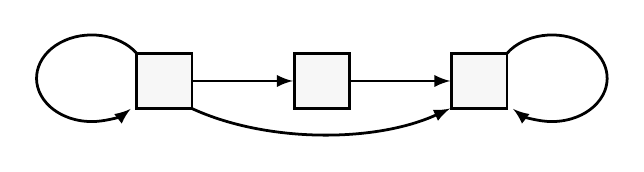
\begin{tikzpicture}
 [line width=1pt, bend angle=45,
 sq/.style={rectangle,inner sep=3pt, minimum size=7mm,
fill=black!3,draw=black}]
\node[sq] (dnode) at (0,0) {$\cchard$};
\node[sq] (fnode) at (2,0) {$\ccharf$};
\node[sq] (bnode) at (4,0) {$\ccharb$};
\draw[-latex] (dnode) -- (fnode);
\draw[-latex] (fnode) -- (bnode);
\draw[-latex] (-0.35,  0.35) arc(35:315:0.7cm and 0.55cm);
\draw[-latex] ( 4.35,  0.35) arc(145:-135:0.7cm and 0.55cm);
\draw[-latex] ( 0.35, -0.35) arc(230:310:2.55cm and 1.4cm);
\end{tikzpicture}\end{center}
\caption{Transitions between types of values in a filesystem}\label{fig_transition}
\end{figure}

In this paper, $n$, $m$ and $o$ denote nodes in $\setn$.
We use $\valf$ for an arbitrary element in $\setf$, 
and by $\valvx$ we mean a value of type $X$ in $\setvx{X}$.

